\begin{figure}
\fbox{
\begin{minipage}{1\linewidth}
\begin{itemize}
\item \textbf{Unit.}
$$
\begin{array}{c}
 \ranked{\Sigma} \ \ \ranked{\leftrightarrow} \ \    \ranked{ \Sigma \cdot 1}\\[5pt]
        {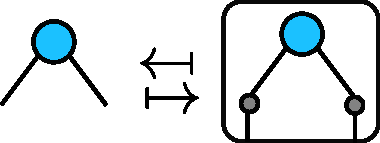
\includegraphics[scale=.4]{pictures/sigma-dot-1}} 
\end{array}
$$
\item \textbf{Associativity.}
$$
\begin{array}{c}
 \ranked{(\Sigma \cdot \Gamma)\cdot \Delta } \ \ \ranked{\to} \ \    \ranked{ \Sigma \cdot (\Gamma \cdot \Delta)}\\[5pt]
        {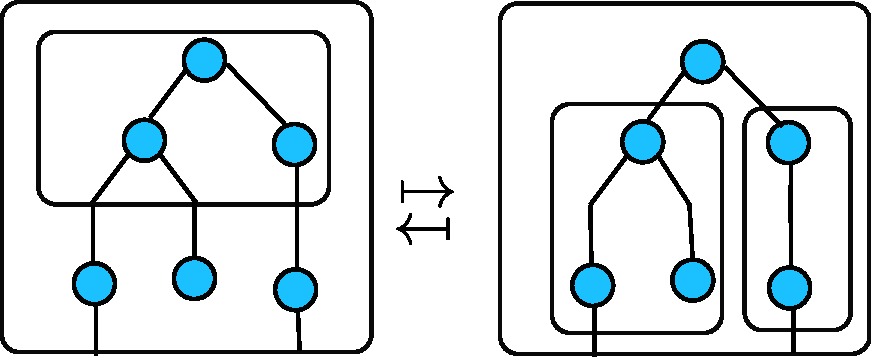
\includegraphics[scale=.4]{pictures/associativity-shallow}} 
\end{array}
$$
\item \textbf{Terms as shallow terms.}
$$
\begin{array}{c}
 \ranked {1 + \shallowterm \Sigma {\tmonad \Sigma}\ \ \to \ \  \tmonad \Sigma}\\[5pt]
        {
        \begin{tabular}{l}
            Every term is either just a port,\\ or has a root and child subterms.    
        \end{tabular}    
        }
\end{array}
$$
\item \textbf{Tensors as shallow terms.}
$$
\begin{array}{c}
\ranked {\Sigma^n \ \ \leftrightarrow \ \ \shallowterm n \Sigma}\\[5pt]
        {
\includegraphics[scale=.4]{pictures/tensor-projection-1}}
\end{array}
$$
\end{itemize}
\end{minipage}
}
\caption{Prime functions for shallow terms.}\label{fig:prime-for-shallow-terms}
\end{figure}

\begin{figure}
\fbox{
\begin{minipage}{1\linewidth}
\begin{itemize}
\item \textbf{Unit.}
$$
\begin{array}{c}
 \ranked{\Sigma \ \ \to \ \ \reduce k \Sigma^k}\\[5pt]
        {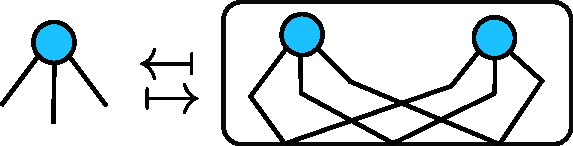
\includegraphics[scale=.4]{pictures/tensor-injection}}
\end{array}
$$
\item \textbf{Increase fold.}
$$
\begin{array}{c}
 \ranked{\reduce k \Sigma \ \ \to \ \ \reduce {k+1}\Sigma}\\[5pt]
        {
\includegraphics[scale=.4]{pictures/add-fold}}	
\end{array}$$
\item \textbf{Decrease fold.}
$$
\begin{array}{c}
 \ranked{\reduce {k+1} \Sigma \ \ \to \ \ \reduce {k}\Sigma+\bot}\\[5pt]
        {
\includegraphics[scale=.4]{pictures/reduce-fold}}	 
\end{array}$$
\item \textbf{projection of copairs.}
$$
\begin{array}{c}
   \ranked{\Sigma\product \Sigma \ \ \to \ \ \reduce 1 \Sigma}\\[5pt]
        {
\includegraphics[scale=.4]{pictures/tensor-projection-1}}	
\end{array}$$
\end{itemize}
\end{minipage}
}
\caption{Additional prime functions for folds.}\label{fig:additional-prime-for-fold}
\end{figure}

\begin{figure}
\fbox{
\begin{minipage}{1\linewidth}
\begin{itemize}
\item \textbf{Folds over pairs.}
$$
\begin{array}{rll}
  \ranked{\reduce k (\Sigma_1 + \Sigma_2)}& \ranked{\to} & \ranked{\reduce k \Sigma_1 + \reduce k \Sigma_2}\\
         (a,i)/f & \mapsto & ((a/f),i)
\end{array}
$$
\item \textbf{Shallow terms over pairs.}
$$
\begin{array}{rll}
  {\shallowterm {(\Sigma_1 + \Sigma_2)} \Gamma} & \ranked{\to} & \ranked{(\shallowterm {\Sigma_1} \Gamma) + (\shallowterm {\Sigma_2} \Gamma)}\\
        (a,i)\tensorpair{t_1,\dots,t_n} &\mapsto& (a\tensorpair{t_1,\dots,t_n},i)
\end{array}
$$
\item \textbf{Shallow terms over copairs.}
$$
\begin{array}{c}
  \ranked{{\shallowterm {(\Sigma_1 \product \Sigma_2)} \Gamma}
   \ \  \to \ \ {(\shallowterm {\Sigma_1} \Gamma) \product (\shallowterm {\Sigma_2} \Gamma)}}\\[5pt]
        {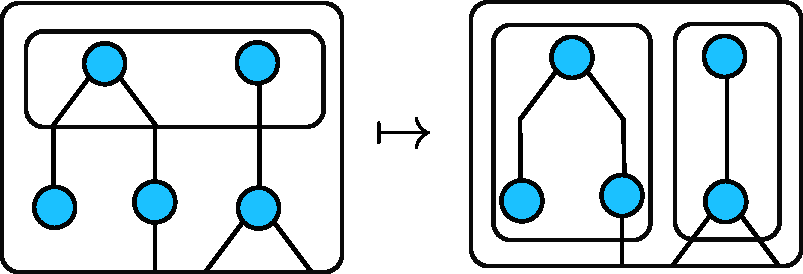
\includegraphics[scale=.4]{pictures/tensor-shallow-distrib}}
        \end{array}
$$
\item \textbf{Folds over copairs.}
$$
\begin{array}{c}
\ranked{(\reduce k \Sigma_1) \product (\reduce k {\Sigma_2}) \ \ \to \ \reduce k (\Sigma_1 \product \Sigma_2)}\\[5pt]
        {
\includegraphics[scale=.4]{pictures/tensor-fold-distrib-2}}  
\end{array}
$$
\item \textbf{Folds over copairs (bis).}
$$
\begin{array}{c}
    \ranked{\reduce k (\Sigma_1 \product \Sigma_2) \ \ \to \ \ \reduce k ((\reduce k {\Sigma_1})\product (\reduce k \Sigma_2))}\\[5pt]
        {
\includegraphics[scale=.4]{pictures/tensor-fold-distrib-1}}   
\end{array}
$$
\item \textbf{Shallow terms over folds.}
$$
\begin{array}{c}
 \ranked{\shallowterm \Sigma {\reduce k \Gamma}\ \ \to \ \ \reduce k (\shallowterm \Sigma {\Gamma})}\\[5pt]
 {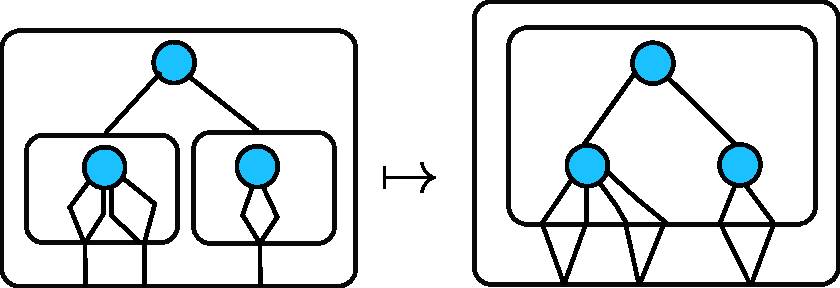
\includegraphics[scale=.4]{pictures/shallow-fold-distrib}} 
\end{array}
$$
\item \textbf{Folds over shallow terms.} 
$$
\begin{array}{c}
 \ranked{\reduce k \Sigma\cdot \Gamma\ \ \to \ \ (\reduce k \Sigma) \cdot \mati k \Gamma}\\[5pt]
 {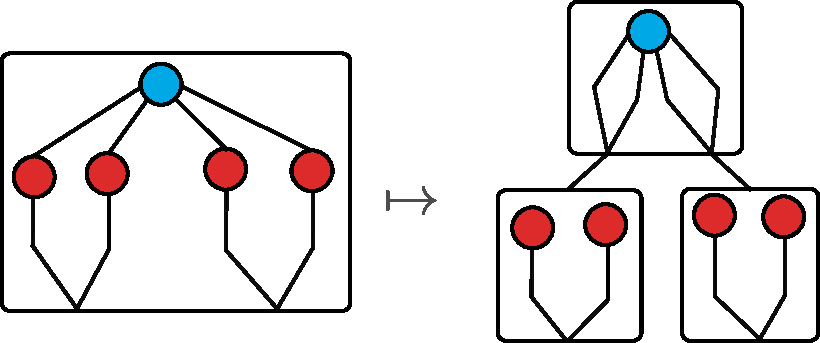
\includegraphics[scale=.4]{pictures/last-prime-function}} 
\end{array}
$$
$\rGamma$ is a set of unary elements.
\end{itemize}
\end{minipage}
}
\caption{Additional distributivity prime functions.} \label{fig:additional-distrib-prime}
\end{figure}

\begin{figure}
\fbox{
\begin{minipage}{1\linewidth}
\begin{itemize}
\item \textbf{Untwist.}
$$
\begin{array}{c}
\ranked{\tmonad {\reduce 1\Sigma} \ \  \to \ \ \reduce 1 \tmonad \Sigma}\\[5pt]
         {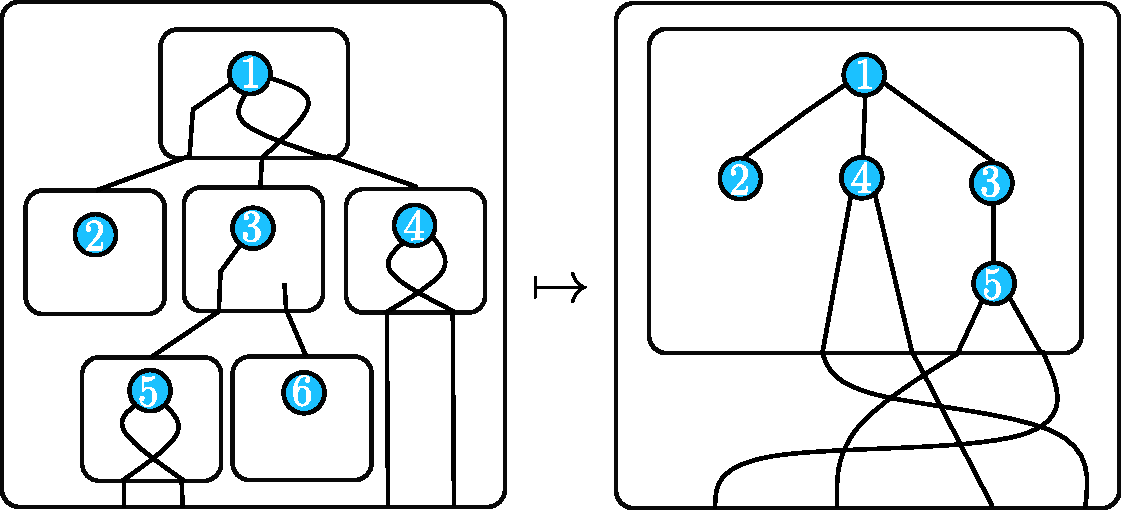
\includegraphics[scale=.4]{pictures/unfold-1}}
\end{array}
$$
\item \textbf{External fold.}
$$
\begin{array}{c}
\ranked{\tmonad {\reduce k\Sigma} \ \  \to \ \ \reduce k \tmonad \reduce k\Sigma}\\[5pt]
         {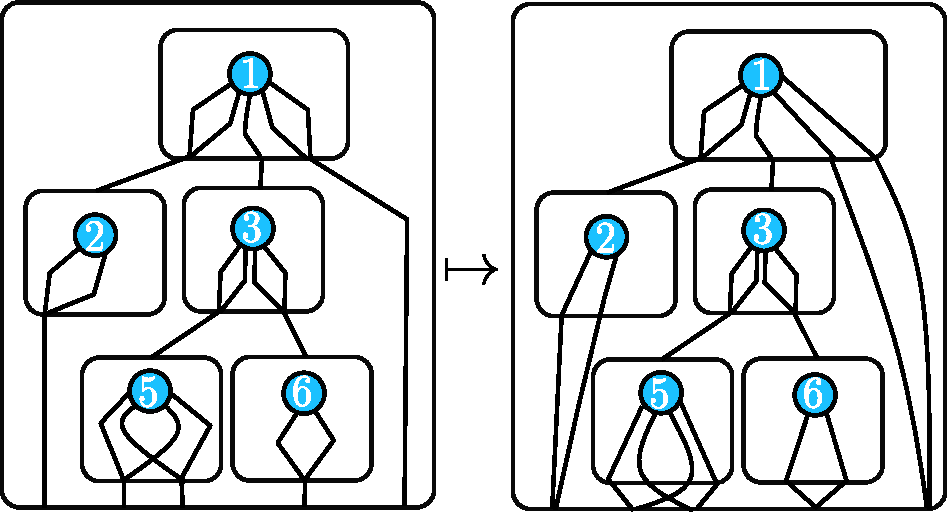
\includegraphics[scale=.43]{pictures/external-unfold-1}}
\end{array}
$$
\item \textbf{Matching.}
$$
\begin{array}{c}
\ranked{\shallowterm {\reduce k \Sigma}{\Gamma^k} \ \ \to \ \ \reduce 1(\shallowterm \Sigma \Gamma)}\\[5pt]
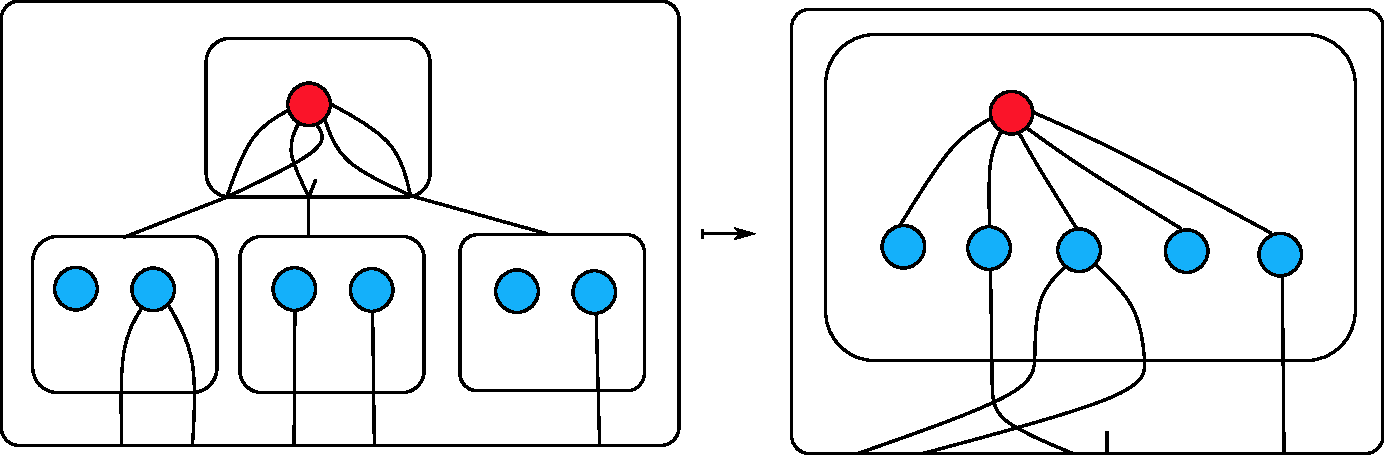
\includegraphics[scale=.3]{pictures/shallow-unfold}
\end{array}
$$
\end{itemize}
\end{minipage}
}
\caption{Weak forms of unfolding.}\label{fig:weak-unfolding}
\end{figure}